\documentclass[12pt,a4paper]{article}
\usepackage[utf8]{inputenc}
\usepackage{amsmath}
\usepackage{amsfonts}
\usepackage{amssymb}
\usepackage{graphicx}
\usepackage[left=3cm,right=3cm,top=2.5cm,bottom=2.5cm]{geometry}

% headers / footers
\usepackage{fancyhdr}
	\pagestyle{fancy}
	\fancyhf{}
	\lhead{ENS1161: Computer Fundamentals}
	\rhead{Assignment 2}
	\lfoot{Martin Ponce, ID: 10371381}
	\rfoot{\thepage\ of \pageref*{LastPage}}
	\renewcommand{\footrulewidth}{0.5pt}

% defining landscape headers / footers
\fancypagestyle{fancylscape}{
	\fancyhf{}
	\renewcommand{\footrulewidth}{0pt}
	\renewcommand{\headrulewidth}{0pt}
	% header
	\begin{textblock}{0.05}[-0.5,-3.185](0,0)
		{\rotatebox{90}{ENS1161: Computer Fundamentals}}
	\end{textblock}
		\begin{textblock}{0.05}[-0.5,-1.08](0,0)
		{\rotatebox{90}{Assignment 2}}
	\end{textblock}
	\begin{textblock}{0.05}[-1,-0.109](0,0)
		{\rotatebox{90}{\rule{24.2cm}{0.5pt}}}
	\end{textblock}
	% footer
	\begin{textblock}{0.05}[-19,-4.28](0,0)
		{\rotatebox{90}{Martin Ponce, ID: 10371381}}
	\end{textblock}
		\begin{textblock}{0.05}[-19,-1.86](0,0)
		{\rotatebox{90}{\thepage\ of \pageref*{LastPage}}}
	\end{textblock}
		\begin{textblock}{0.05}[-18.7,-0.109](0,0)
		{\rotatebox{90}{\rule{24.2cm}{0.5pt}}}
	\end{textblock}
}

% defining settings for textpos
\usepackage[absolute]{textpos}
\setlength{\TPHorizModule}{\paperwidth}
\setlength{\TPVertModule}{\paperheight}

% creates landscape pages
\usepackage{pdflscape}

% add pages from pdfs
\usepackage{pdfpages}

% adds links to references and colors them blue
\usepackage[bookmarksdepth=3]{hyperref}
\hypersetup{colorlinks=true,
			linkcolor=blue,
			citecolor=blue,
			urlcolor=blue}

% adjusts padding between caption and figure
\setlength{\belowcaptionskip}{10pt}

% last page
\usepackage{lastpage}

% front matter
\title{Edith Cowan University\\ENS1161: Computer Fundamentals\\Assignment 2}
\author{Martin Ponce\\ID: 10371381}
\date{\today}
\setcounter{tocdepth}{2}

\begin{document}

% assignment coversheet
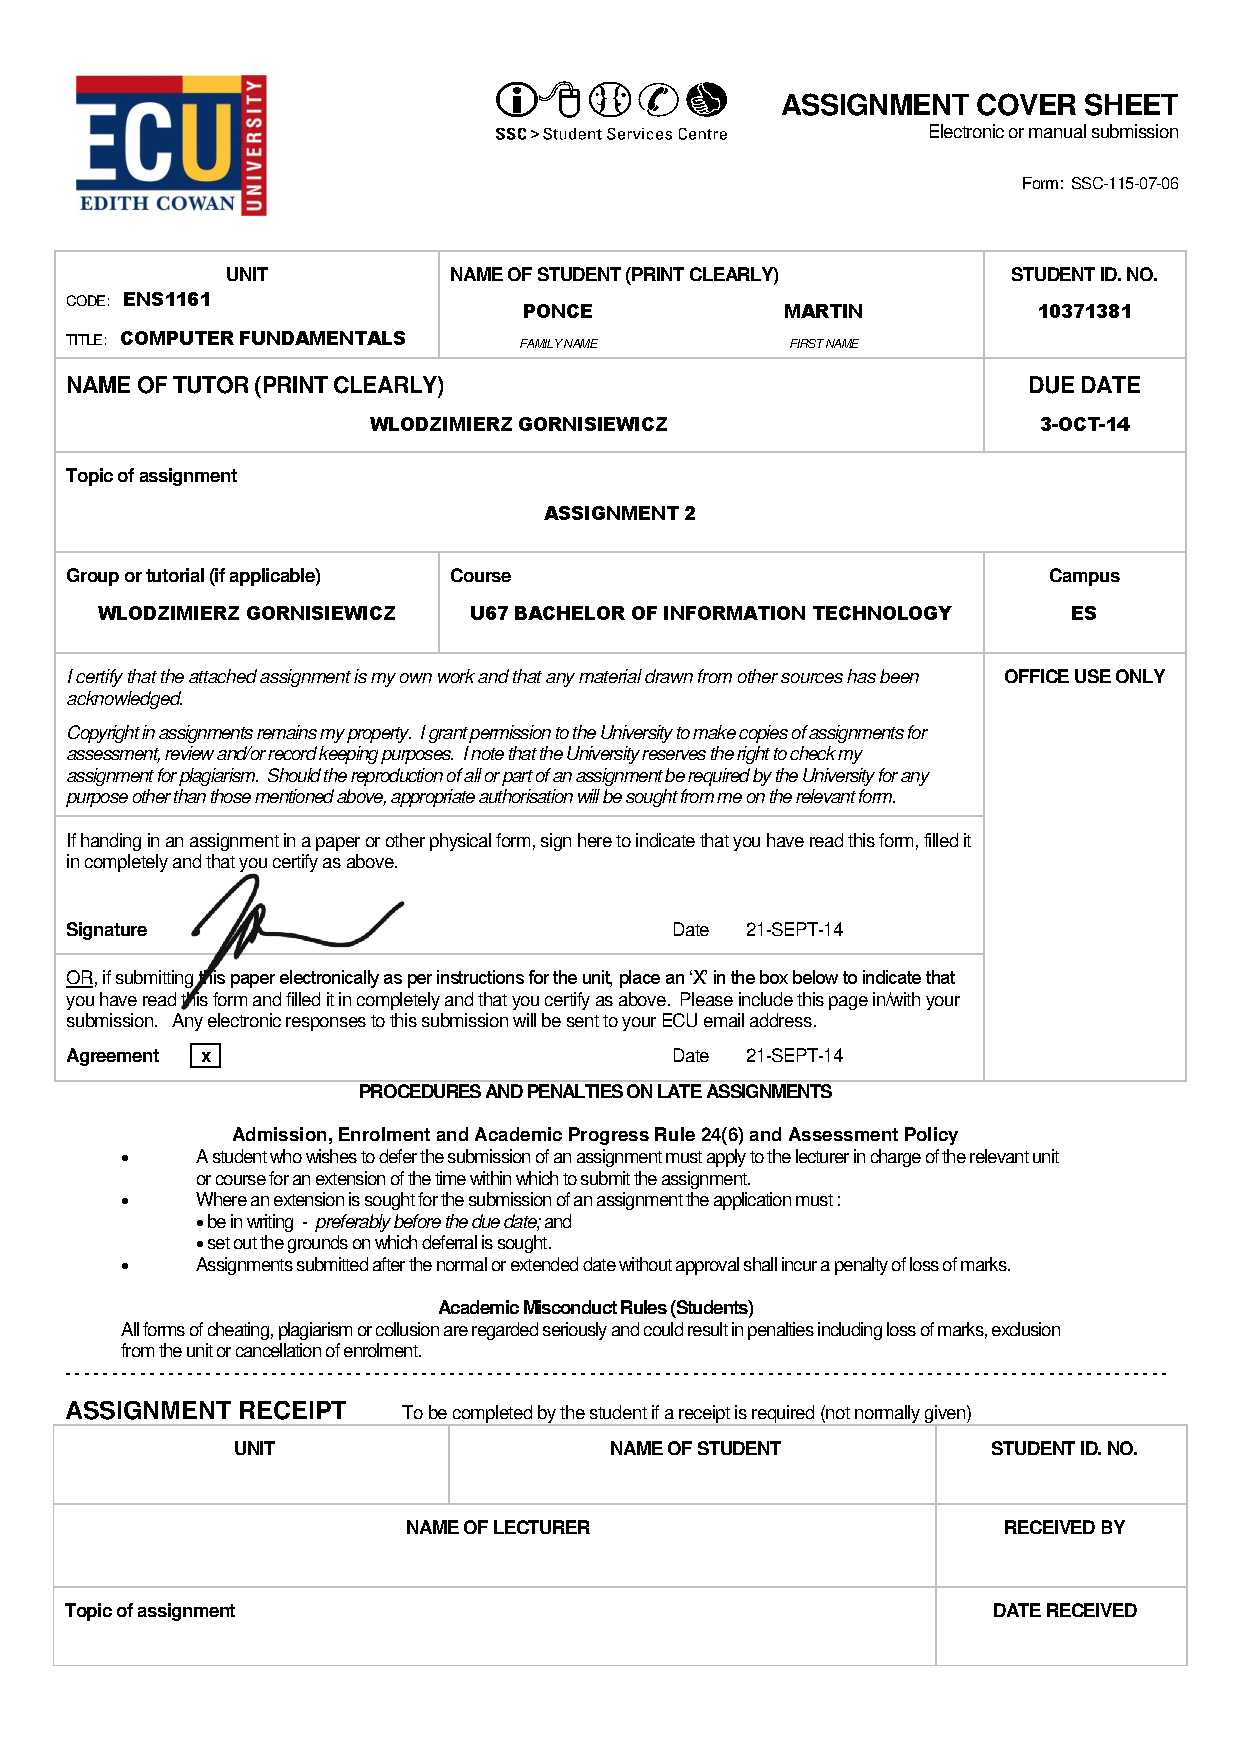
\includepdf{./img/assignment_coversheet_PONCE_10371381.pdf}

% title page
\newpage
\null  % Empty line
\nointerlineskip  % No skip for prev line
\vfill
\let\snewpage \newpage
\let\newpage \relax
\maketitle
\thispagestyle{empty}
\let \newpage \snewpage
\vfill

% toc
\newpage
\tableofcontents

% page 1
\newpage
\section{Question 1}

Consider the functions $f$, $g$ and $h$, all defined on the set \{0, 1, 2, 3, ..., 12\}.

\begin{table}[!h]
\centering
\caption{$f(x)$}
\begin{tabular}{r|c|c|c|c|c|c|c|c|c|c|c|c|c}
$x$ & 0 & 1 & 2 & 3 & 4 & 5 & 6 & 7 & 8 & 9 & 10 & 11 & 12 \\
\hline
$f(x)$ & 0 & 5 & 10 & 4 & 3 & 1 & 12 & 7 & 11 & 9 & 2 & 8 & 6
\end{tabular}
\end{table}

\begin{table}[!h]
\centering
\caption{$g(x)$}
\begin{tabular}{r|c|c|c|c|c|c|c|c|c|c|c|c|c}
$x$ & 0 & 1 & 2 & 3 & 4 & 5 & 6 & 7 & 8 & 9 & 10 & 11 & 12 \\
\hline
$g(x)$ & 5 & 4 & 11 & 0 & 6 & 10 & 2 & 7 & 1 & 12 & 9 & 8 & 3
\end{tabular}
\end{table}

\begin{table}[!h]
\centering
\caption{$h(x)$}
\begin{tabular}{r|c|c|c|c|c|c|c|c|c|c|c|c|c}
$x$ & 0 & 1 & 2 & 3 & 4 & 5 & 6 & 7 & 8 & 9 & 10 & 11 & 12 \\
\hline
$h(x)$ & 3 & 6 & 0 & 10 & 9 & 5 & 2 & 12 & 1 & 7 & 11 & 4 & 8
\end{tabular}
\end{table}

\subsection{Write down the values of: $g(f(h(7)))$ \& $h^{-1}(g^{-1}(3))$}

\begin{align*}
g(f(h(7))) &= 2 \\
\\
h(7) &= 12 \\
f(12) &= 6 \\
g(6) &= 2
\end{align*}

\begin{align*}
h^{-1}(g^{-1}(3)) &= 7 \\
\\
g^{-1}(3) &= 12 \\
h^{-1}(12) &= 7
\end{align*}

\subsection{Construct a table of values for $h(g^{-1}(x))$}

\begin{table}[!h]
\centering
\caption{$h(g^{-1}(x))$}
\begin{tabular}{r|c|c|c|c|c|c|c|c|c|c|c|c|c}
$x$ & 0 & 1 & 2 & 3 & 4 & 5 & 6 & 7 & 8 & 9 & 10 & 11 & 12 \\
\hline
$h(g^{-1}(x))$ & 10 & 1 & 2 & 8 & 6 & 3 & 9 & 12 & 4 & 11 & 5 & 0 & 7
\end{tabular}
\end{table}

\newpage
\subsection{Construct a table for $f(f(x))$}

What can you conclude about the inverse of $f$?

Function $f(x)$ is it's own inverse, or involution.

\begin{table}[!h]
\centering
\caption{$f(f(x))$}
\begin{tabular}{r|c|c|c|c|c|c|c|c|c|c|c|c|c}
$x$ & 0 & 1 & 2 & 3 & 4 & 5 & 6 & 7 & 8 & 9 & 10 & 11 & 12 \\
\hline
$f(f(x))$ & 0 & 1 & 2 & 3 & 4 & 5 & 6 & 7 & 8 & 9 & 10 & 11 & 12
\end{tabular}
\end{table}

\subsection{Construct a table for $h^{-1}(x)$, and draw its graph}

\begin{table}[!h]
\centering
\caption{$h^{-1}(x)$}
\begin{tabular}{r|c|c|c|c|c|c|c|c|c|c|c|c|c}
$x$ & 0 & 1 & 2 & 3 & 4 & 5 & 6 & 7 & 8 & 9 & 10 & 11 & 12 \\
\hline
$h^{-1}(x)$ & 2 & 8 & 6 & 0 & 11 & 5 & 1 & 9 & 12 & 4 & 3 & 10 & 7
\end{tabular}
\end{table}

\begin{figure}[h]
\centering
\caption{$h^{-1}(x)$ graph}
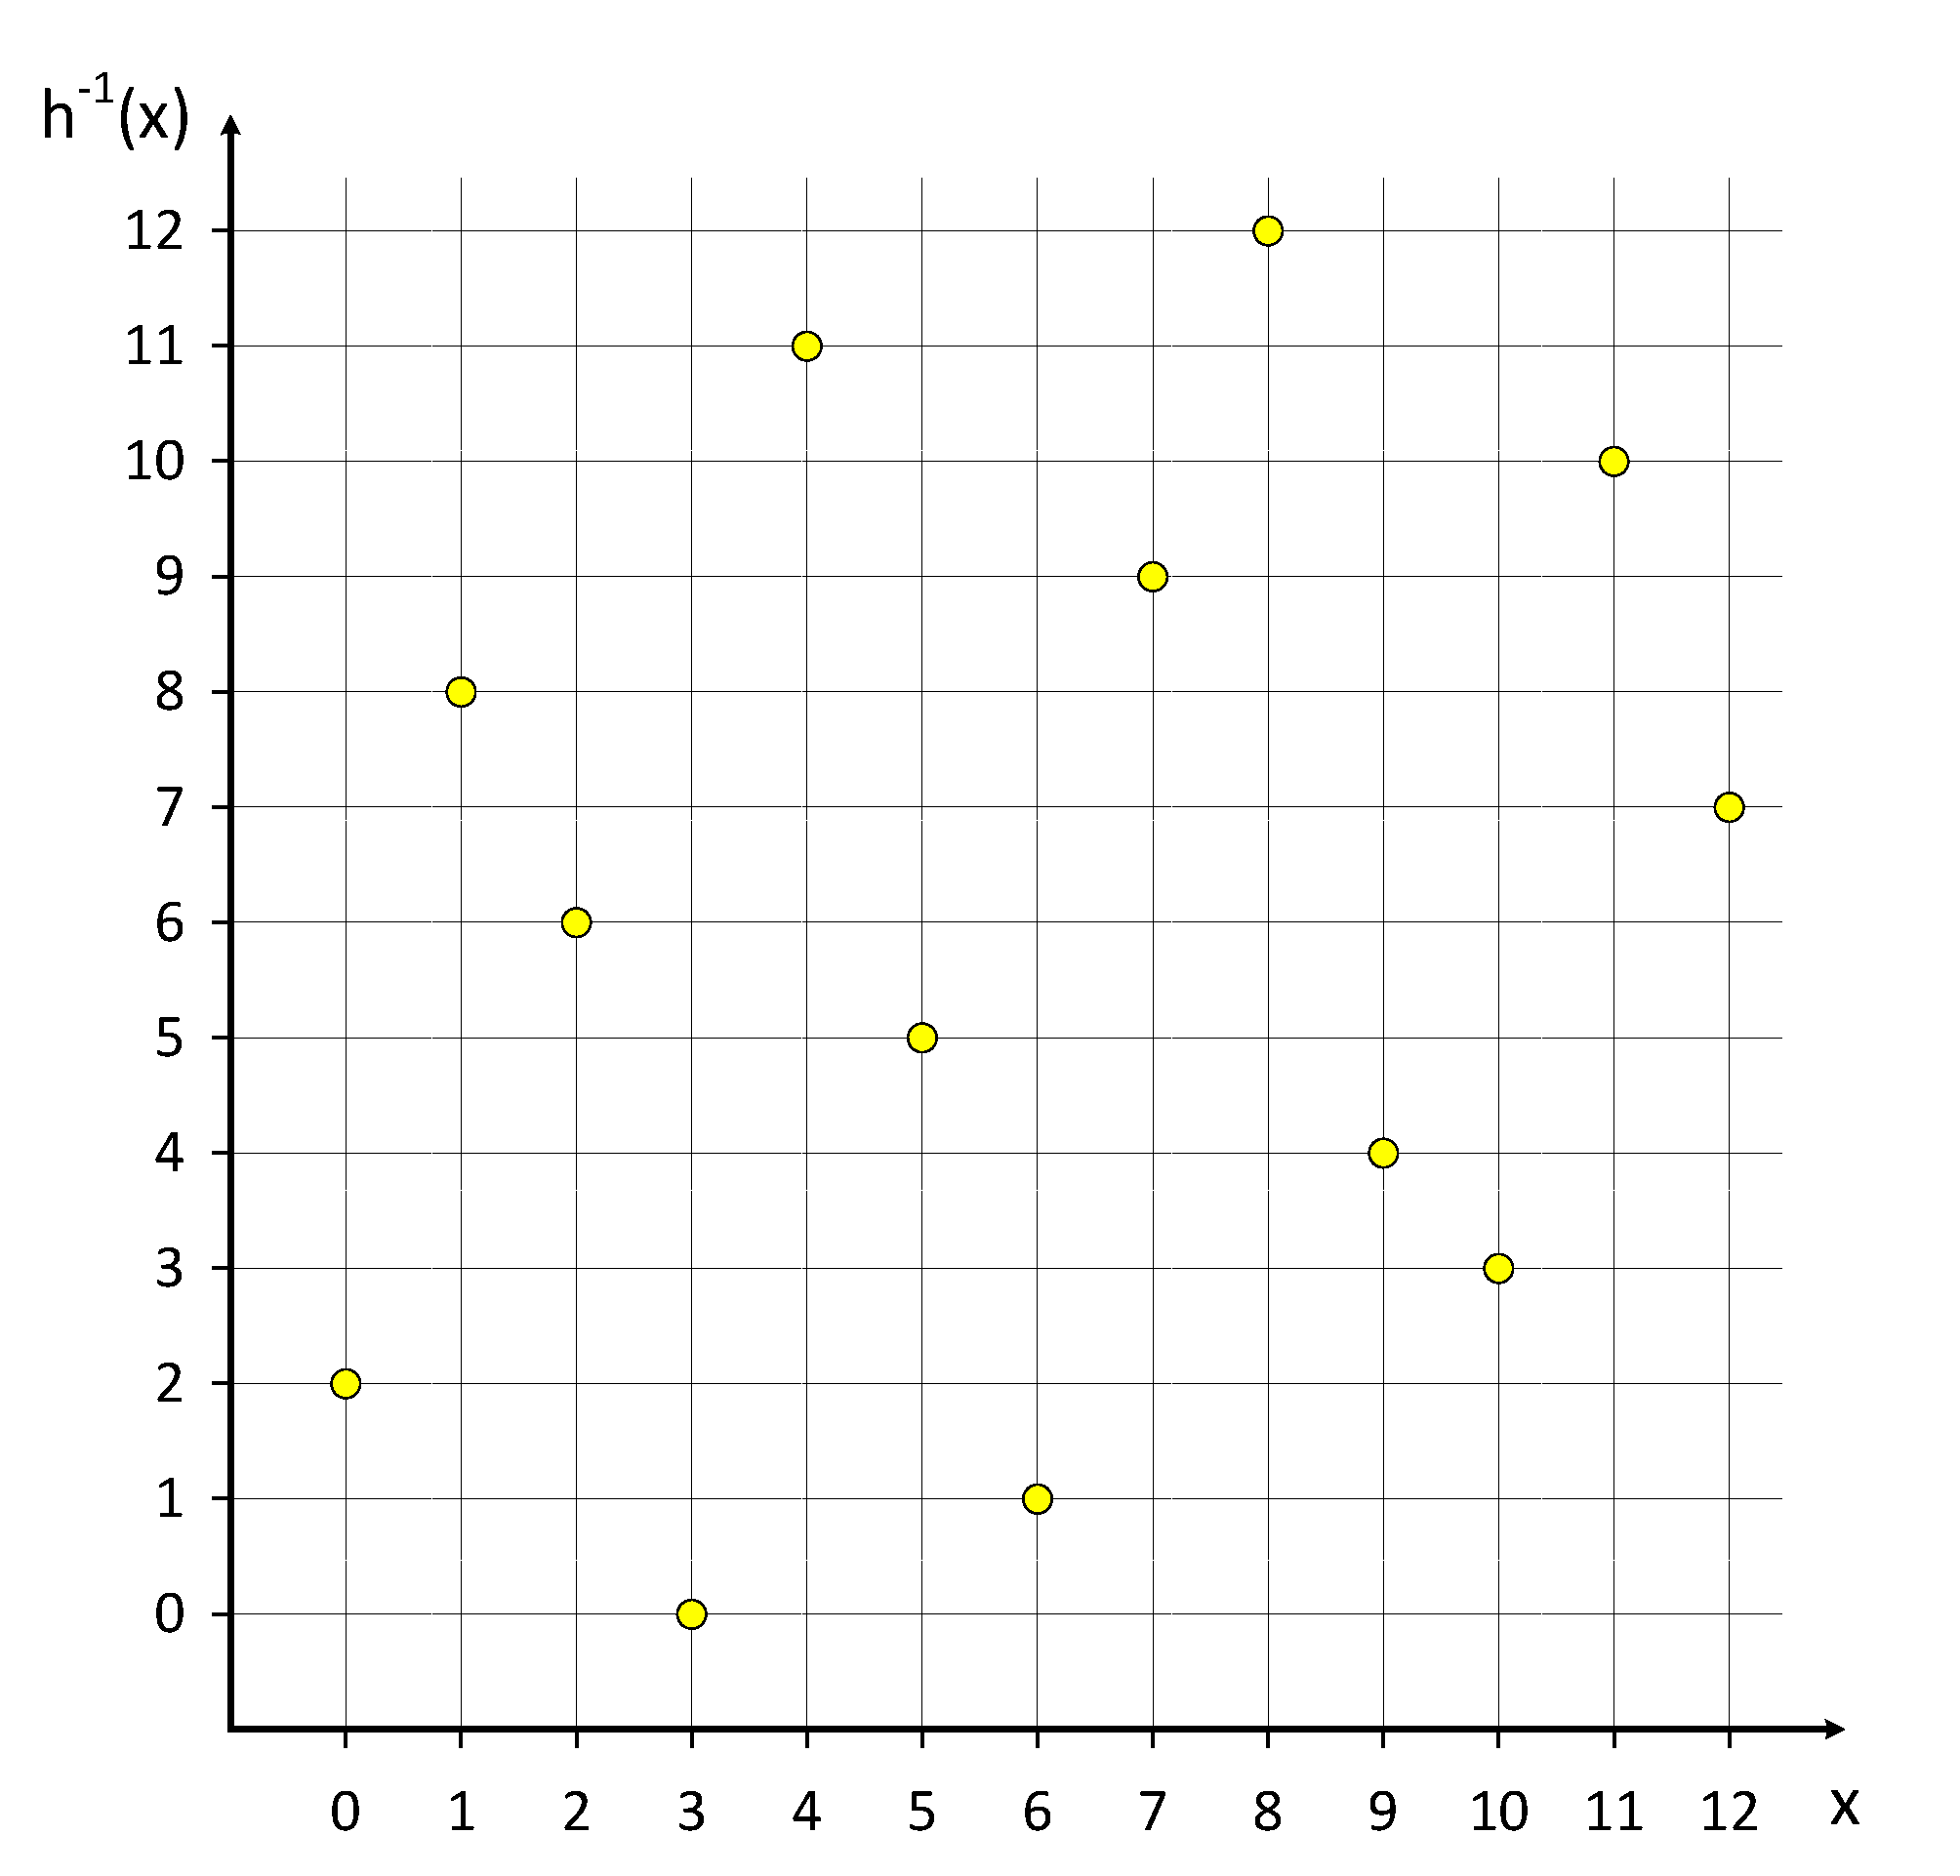
\includegraphics[scale=0.35]{./img/graph_q1-4.pdf}
\end{figure}

\section{Question 2}

Suppose there is a set of growers $G = \{a, b, c, d\}$, a set of retailers $R = \{e, f, g\}$, and a set of customers $C = \{m, n, p, q, r\}$. \\
\\
There are two relations $A$ and $B$ on $G \times R$ and $R \times C$ respectively, defined by: \\
\\
$aAe, aAg, bAf, cAf, cAg, dAe$ and $eBn, eBq, fBp, gBm, gBr$ \\
\\
$xAy$ means ``grower $x$ sold goods to retailer $y$'', and \\ \noindent
$yA^{-1}x$ means ``retailer $y$ bought goods from grower $x$''

\subsection{Find the matrices $M(A)$ and $M(B)$ that represent the relations $A$ and $B$}

\begin{figure}[h]
\centering
\caption{$M(A)$ and $M(B)$ matrices}
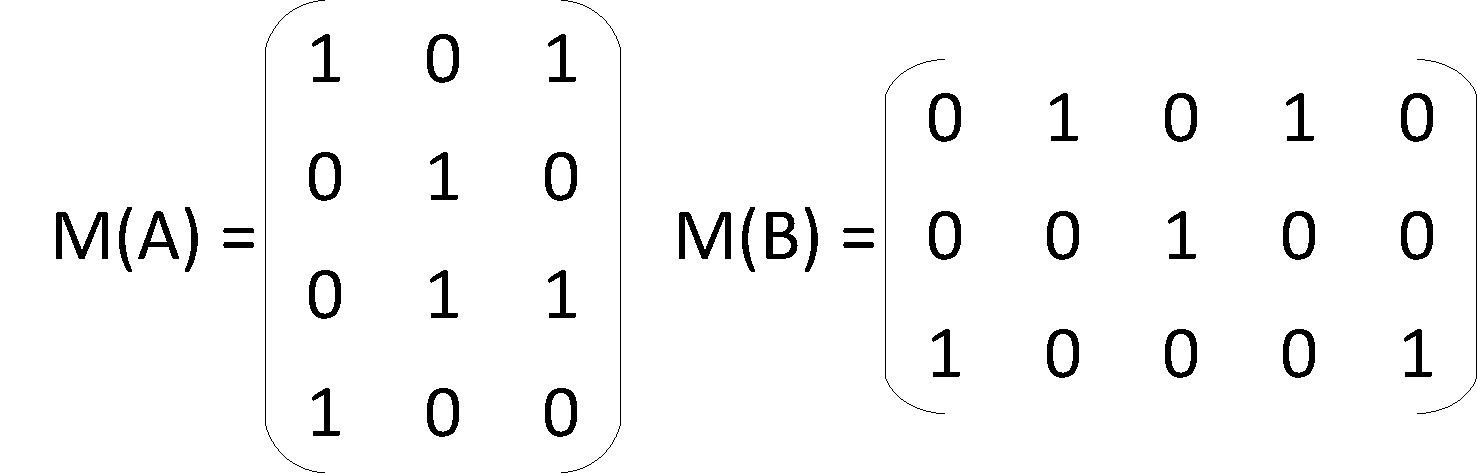
\includegraphics[scale=0.35]{./img/matrix_q2-1.pdf}
\end{figure}

\subsection{Find the matrices $M(A)^T$ and $M(B)^T$ that represent the relations $A^{-1}$ and $B^{-1}$}

\begin{figure}[h]
\centering
\caption{$M(A)^T$ and $M(B)^T$ matrices}
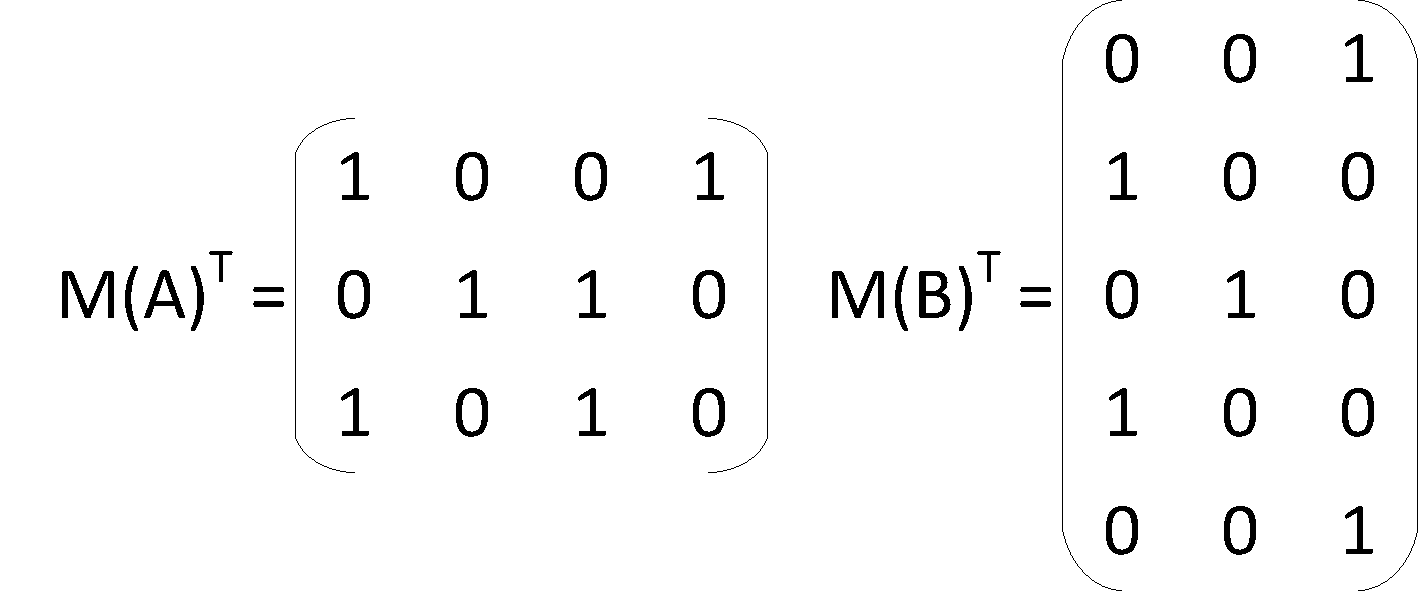
\includegraphics[scale=0.35]{./img/matrix_q2-2.pdf}
\end{figure}

\newpage
\subsection{Consider the two queries}

Which customers have received goods that came from the same grower/s as those goods received by A: customer $p$? B: customer $q$? \\
\\
Find the logical matrix products $M(A)M(B)$ and then $M(B)^TM(A)^T$, and finally $M(B)^TM(A)^TM(A)M(B)$, and hence answer the queries.

\begin{figure}[h]
\centering
\caption{$M(A)M(B)$ and $M(B)^TM(A)^T$ matrices}
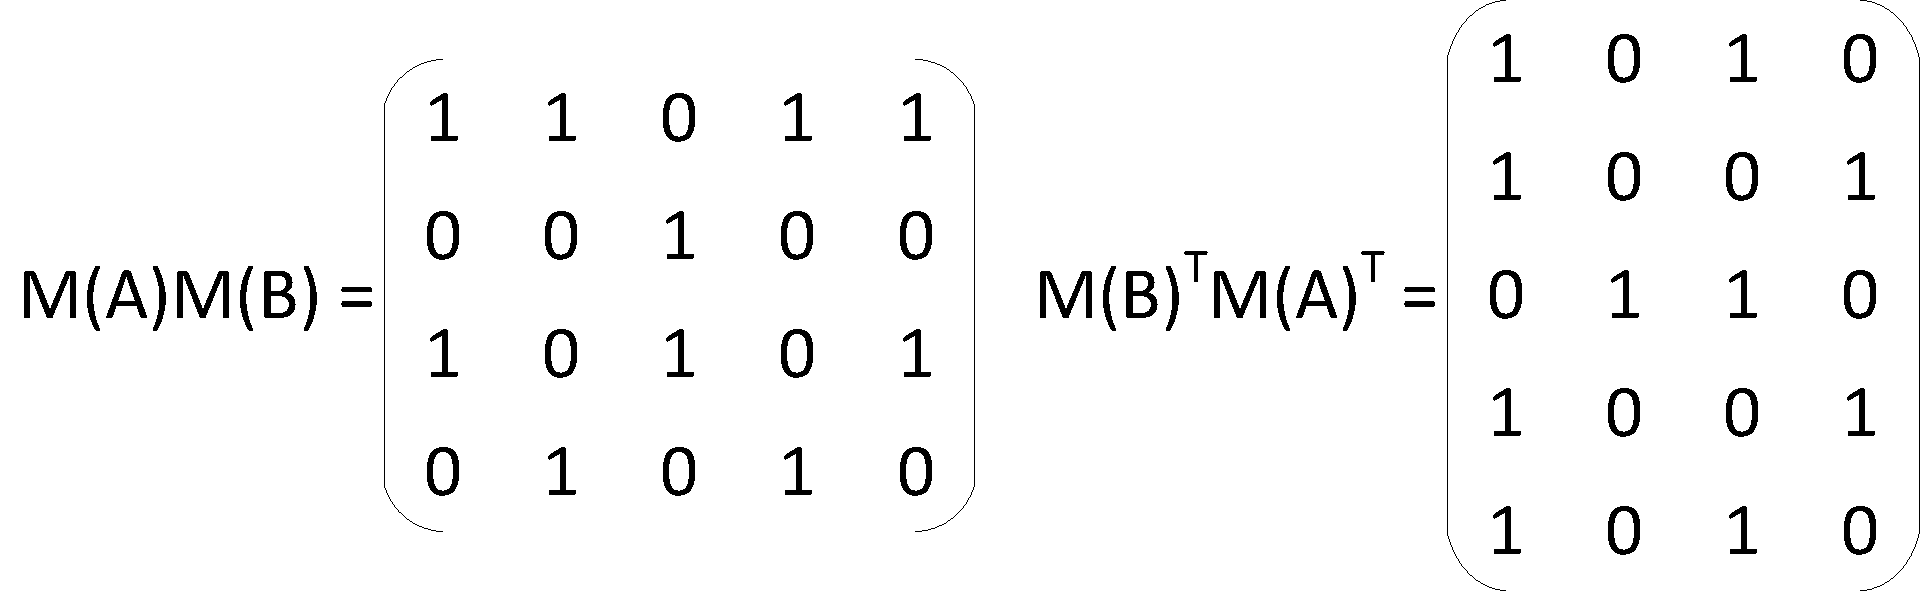
\includegraphics[scale=0.35]{./img/matrix_q2-3A.pdf}
\end{figure}

\begin{figure}[h]
\centering
\caption{$M(B)^TM(A)^TM(A)M(B)$ matrix}
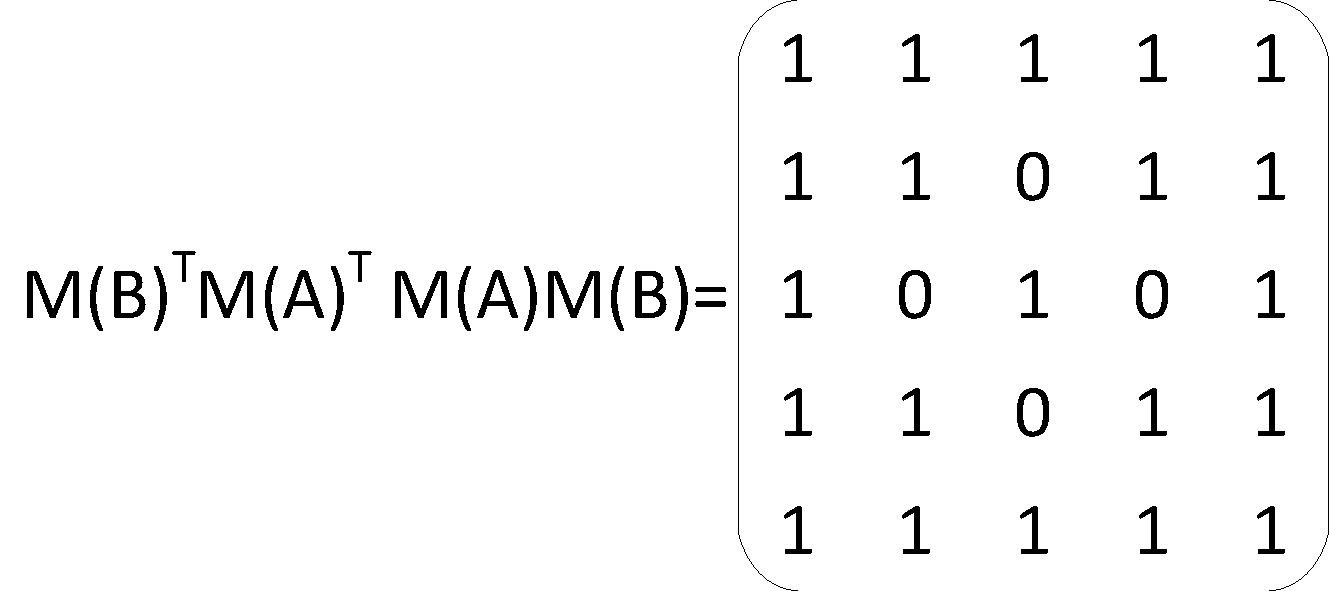
\includegraphics[scale=0.35]{./img/matrix_q2-3B.pdf}
\end{figure}

\subsubsection{A: Customer $p$}

Customers $p$, $m$ and $r$ received goods from Growers $b$ and $c$.

\subsubsection{B: Customer $q$}

Customers $q$, $m$, $n$ and $r$ received goods from Growers $a$ and $d$.

\newpage
\section{Question 3}

\subsection{A: Base number conversion}

Consider the following table:

\begin{figure}[h]
\centering
\caption{Question 3 table}
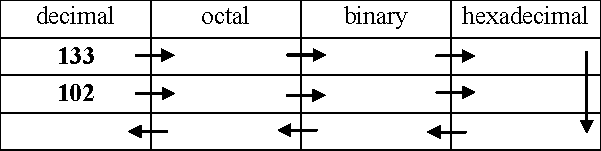
\includegraphics[scale=1]{./img/table_q3-A.pdf}
\end{figure}

\subsubsection{Convert each of the decimal numbers in the first column to octal}

\begin{table}[!h]
\centering
\caption{Decimal to octal}
\begin{tabular}{c|c|c|c}
Decimal & Octal & Binary & Hexadecimal \\
\hline
$133_{10}$ & $205_{8}$ &  &  \\
\hline
$102_{10}$ & $146_{8}$ &  &  \\
\hline
  &  &  &
\end{tabular}
\end{table}

\subsubsection{Convert the two octal numbers to binary}

\begin{table}[!h]
\centering
\caption{Octal to binary}
\begin{tabular}{c|c|c|c}
Decimal & Octal & Binary & Hexadecimal \\
\hline
$133_{10}$ & $205_{8}$ & $1000$ $0101_{2}$ &  \\
\hline
$102_{10}$ & $146_{8}$ & $0110$ $0110_{2}$ &  \\
\hline
  &  &  &
\end{tabular}
\end{table}

\subsubsection{Convert the two binary numbers to hexadecimal}

\begin{table}[!h]
\centering
\caption{Binary to hexadecimal}
\begin{tabular}{c|c|c|c}
Decimal & Octal & Binary & Hexadecimal \\
\hline
$133_{10}$ & $205_{8}$ & $1000$ $0101_{2}$ & $85_{16}$ \\
\hline
$102_{10}$ & $146_{8}$ & $0110$ $0110_{2}$ &  $66_{16}$ \\
\hline
  &  &  &
\end{tabular}
\end{table}

\newpage
\subsubsection{Add the two hexadecimal numbers}

\begin{table}[!h]
\centering
\caption{Hexadecimal sum}
\begin{tabular}{c|c|c|c}
Decimal & Octal & Binary & Hexadecimal \\
\hline
$133_{10}$ & $205_{8}$ & $1000$ $0101_{2}$ & $85_{16}$ \\
\hline
$102_{10}$ & $146_{8}$ & $0110$ $0110_{2}$ &  $66_{16}$ \\
\hline
  &  &  & EB$_{16}$
\end{tabular}
\end{table}

\subsubsection{Convert the hexadecimal sum to binary, then to octal and then to decimal}

\begin{table}[!h]
\centering
\caption{Sum to binary, octal and decimal}
\begin{tabular}{c|c|c|c}
Decimal & Octal & Binary & Hexadecimal \\
\hline
$133_{10}$ & $205_{8}$ & $1000$ $0101_{2}$ & $85_{16}$ \\
\hline
$102_{10}$ & $146_{8}$ & $0110$ $0110_{2}$ &  $66_{16}$ \\
\hline
$235_{10}$ & $353_{8}$ & $1110$ $1011_{2}$ & EB$_{16}$
\end{tabular}
\end{table}

\subsection{B: Fractions}

\subsubsection{Convert the decimal fraction 0.21875 to binary}

\begin{align*}
0.21875 * 2 &= 0.4375 \\
0.4375 * 2 &= 0.875 \\
0.875 * 2 &= 1.75 \\
0.75 * 2 &= 1.5 \\
0.5 * 2 &= 1.0 \\
\\
0.21875_{10} &= 0.00111_{2}
\end{align*}

\subsubsection{Convert the decimal fraction 0.40625 to binary}

\begin{align*}
0.40625 * 2 &= 0.8125 \\
0.8125 * 2 &= 1.625 \\
0.625 * 2 &= 1.25 \\
0.25 * 2 &= 0.5 \\
0.5 * 2 &= 1.0 \\
\\
0.40625_{10} &= 0.01101_{2}
\end{align*}

\newpage
\subsubsection{Add the two binary fractions from 3.2.1 and 3.2.2}

\begin{equation*}
\centering
\begin{array}{c c c c c c c}
  & 1 & 1 & 1 & 1 &   & carry \\
  & 0 & 0 & 1 & 1 & 1         \\
+ & 0 & 1 & 1 & 0 & 1         \\ \hline
0.& 1 & 0 & 1 & 0 & 0
\end{array}
\end{equation*}

\subsubsection{Convert the binary fraction from 3.2.3 to decimal}

\begin{align*}
10100_{2} &= 20_{10} \\
\\
20_{10} * 2^{5} &= 0.625_{10} \\
\\
0.10100_{2} &= 0.625_{10} \\
\\
0.21875_{10} + 0.40625_{10} &= 0.625_{10}
\end{align*}

\subsection{C: Addition}

Add the following, given that 3.3.1 is binary, 3.3.2 is octal and 3.3.3 is hexadecimal:

\subsubsection{Binary addition}

\begin{equation*}
\centering
\begin{array}{c c c c c c c c c c}
  & 1 & 0 & 0 & 0 & 0 & 1 & 1 &   & carry \\
  &   & 1 & 0 & 0 & 1 & 0 & 1 & 1 &       \\
+ &   & 1 & 1 & 0 & 0 & 0 & 1 & 1 &	      \\ \hline
  & 1 & 0 & 1 & 0 & 1 & 1 & 1 & 0 &
\end{array}
\end{equation*}

\subsubsection{Octal addition}

\begin{equation*}
\centering
\begin{array}{c c c c c c c}
  & 1 & 1 & 1 & 1 &   & carry \\
  &   & 3 & 3 & 7 & 5 &       \\
+ &   & 6 & 7 & 4 & 3 &       \\ \hline
  & 1 & 2 & 3 & 4 & 0 &
\end{array}
\end{equation*}

\subsubsection{Hexadecimal addition}

\begin{equation*}
\centering
\begin{array}{c c c c c c c c}
  &   & 1 & 1 & 0 & 0 &   & carry \\
  &   & 3 & D & E & 8 & C &       \\
+ &   & 7 & A & 5 & 5 & 2 &       \\ \hline
  &   & B & 8 & 3 & D & E &
\end{array}
\end{equation*}

\newpage
\subsection{D: BCD additions}

Perform ``BCD additions'' on the following pairs of hexadecimal numbers. Show all your working.

\subsubsection{23267 + 49684}

\begin{equation*}
\centering
\begin{array}{c c c c c c c c}
  &   & 1 & 0 & 1 & 1 &   & carry \\
  &   & 2 & 3 & 2 & 6 & 7 &       \\
+ &   & 4 & 9 & 6 & 8 & 4 &       \\ \hline
  &   & 7 & C & 9 & F & B &       \\
+ &   & 0 & 6 & 0 & 6 & 6 &       \\ \hline
  &   & 7 & 2 & 9 & 5 & 1 &
\end{array}
\end{equation*}

\subsubsection{592778 + 183983}

\begin{equation*}
\centering
\begin{array}{c c c c c c c c c}
  &   & 1 & 0 & 1 & 1 & 1 &   & carry \\
  &   & 5 & 9 & 2 & 7 & 7 & 8 &       \\
+ &   & 1 & 8 & 3 & 9 & 8 & 3 &       \\ \hline
  &   & 7 & 1 & 6 & 1 & 0 & B &       \\
+ &   & 0 & 6 & 0 & 6 & 6 & 6 &       \\ \hline
  &   & 7 & 7 & 6 & 7 & 6 & 1 &       \\
\end{array}
\end{equation*}

\section{Question 4}

For each of the following, suppose that two 8-bit binary numbers have been added. In each case the 8-bit output is given and the values of the N, V and C flags. For each case give the correct answer as a decimal number: \\
\\
A: If the result is interpreted as the sum of \textbf{unsigned} integers \\
\\
B: If the result is interpreted as the sum of \textbf{signed} integers.

\begin{table}[!h]
\centering
\caption{8-bit output}
\begin{tabular}{c|c|c|c|c}
  & 8-bit output & N & V & C \\ \hline
1 & 1100 0000 & 1 & 1 & 0 \\ \hline
2 & 0011 1111 & 0 & 1 & 1 \\ \hline
3 & 0010 1011 & 0 & 0 & 1 \\ \hline
4 & 1100 1010 & 1 & 0 & 0 \\ \hline
5 & 1100 1011 & 1 & 0 & 1
\end{tabular}
\end{table}

\newpage
\subsection{1100 0000}

\subsubsection{Unsigned}

1100 0000 with flag C = 0: 8-bit output.

\begin{align*}
&\ 1100\ 0000_{2}    \\
=&\ \text{C}0_{16} \\
=&\ 192_{10}
\end{align*}

\subsubsection{Signed}

1100 0000 with flags N = 1 and V = 1: Positive 16-bit output.

\begin{align*}
&\ 0000\ 0000\ 1100\ 0000_{2} \\
=&\ 00\text{C}0_{16} \\
=&\ +192_{10}
\end{align*}

\subsection{0011 1111}

\subsubsection{Unsigned}

0011 1111 with flag C = 1: 16-bit output

\begin{align*}
&\ 0000\ 0001\ 0011\ 1111_{2} \\
=&\ 1\text{3F}_{16} \\
=&\ 319_{10}
\end{align*}

\subsubsection{Signed}

0011 1111 with flags N = 0 and V = 1: Negative 16-bit output.

\begin{align*}
&\ 1111\ 1111\ 0011\ 1111_{2} \\
\text{1's complement} =&\ 0000\ 0000\ 1100\ 0000_{2} \\
+ 1 =&\ 0000\ 0000\ 1100\ 0001_{2} \\
=&\ \text{C}1_{16} \\
=&\ -193_{10}
\end{align*}

\subsection{0010 1011}

\subsubsection{Unsigned}

0010 1011 with flag C = 1: 16-bit output

\begin{align*}
&\ 0000\ 0001\ 0010\ 1011_{2} \\
=&\ 12\text{B}_{16} \\
=&\ 299_{10}
\end{align*}

\subsubsection{Signed}

0010 1011 with flags N = 0 and V = 0: Positive 8-bit output.

\begin{align*}
&\ 0010\ 1011_{2} \\
=&\ 2\text{B}_{16} \\
=&\ +43_{10}
\end{align*}

\subsection{1100 1010}

\subsubsection{Unsigned}

1100 1010 with flag C = 0: 8-bit output

\begin{align*}
&\ 1100\ 1010_{2} \\
=&\ \text{CA}_{16} \\
=&\ 202_{10}
\end{align*}

\subsubsection{Signed}

1100 1010 with flags N = 1 and V = 0: Negative 8-bit output.

\begin{align*}
&\ 1100\ 1010_{2} \\
\text{1's complement} =&\ 0011\ 0101_{2} \\
+ 1 =&\ 0011\ 0110_{2} \\
=&\ 36_{16} \\
=&\ -54_{10}
\end{align*}

\subsection{1100 1011}

\subsubsection{Unsigned}

1100 1011 with flag C = 1: 16-bit output.

\begin{align*}
&\ 0000\ 0001\ 1100\ 1011_{2} \\
=&\ 1\text{CB}_{16} \\
=&\ 459_{10}
\end{align*}

\newpage
\subsubsection{Signed}

1100 1011 with flag N = 1 and V = 0: Negative 8-bit output.

\begin{align*}
&\ 1100\ 1011_{2} \\
\text{1's complement} =&\ 0011\ 0100_{2} \\
+ 1 =&\ 0011\ 0101_{2} \\
=&\ 35_{16} \\
=&\ -53_{10}
\end{align*}

\subsection{Question 5}

\begin{table}[!h]
\centering
\caption{Question 5 answers}
\begin{tabular}{c|c|c|c|c}
No. & Cols in array & Row No. & Col No. & Seq. Pos. \\
\hline
1 & 14 &  5 & 11 & 154 \\ \hline
2 & 36 &  1 & 27 &  27 \\ \hline
3 &  9 &  4 &  8 &  35 \\ \hline
4 & 28 & 17 & 11 & 459 \\ \hline
5 & 30 &  4 &  8 &  98 \\ \hline
6 & 45 &  7 & 30 & 300 \\ \hline
7 & 24 &  4 & 13 &  85 \\ \hline
\end{tabular}
\end{table}

\end{document}